\documentclass[NET,english,aspectratio=169,notitleframe]{tumbeamer}

%settings
\usepackage[utf8]{inputenc}
\usepackage{pgfplotstable}
\usepackage{marvosym}
\usepackage{filecontents}
\usepackage{packages}
\usepackage{beamermods}

\usepackage[backend=bibtex, style=ieee]{biblatex}

\usepackage{csquotes}

\usetikzlibrary{calc}
\usetikzlibrary{arrows.meta}


% For lecture mode (use package option 'lecture'):
%\lecture[GRNVS]{Grundlagen Rechnernetze und Verteilte Systeme}
%\module{IN0010}
%\semester{SoSe\,2016}
%\assistants{Johannes Naab, Stephan Günther, Maurice Leclaire}

\usepackage{pgfplots}
\pgfplotsset{compat=newest}
\usepackage{tumcolor}
\usepackage{tumcolors}
\usepackage{textpos}


\usepackage{pgfpages}
\usepackage{ifthen}
% ============================================================================
% jobname solution
% ============================================================================
\newif\ifsolution%
\ifthenelse{\equal{\detokenize{notes}}{\jobname}}{%
\setbeameroption{show notes on second screen=bottom}
\setbeamercolor{note page}{bg=white, fg=black}
\setbeamercolor{note title}{bg=white!95!black, fg=black}
}{
}

%\xdefinecolor{orange}{cmyk}{0,0.65,0.95,0} 
%\xdefinecolor{dblue}{cmyk}{1,0.54,0.04,0.19}
%\xdefinecolor{blue}{cmyk}{1,0.43,0,0}  
%\xdefinecolor{lblue}{cmyk}{0.65,0.19,0.01,0.04}
%\xdefinecolor{green} {cmyk}{0.35,0,1,0.2} 
%xdefinecolor{yellow}{rgb}{1.00,0.71,0.00} 
%\colorlet{lgtorange}{orange!20} 
%\colorlet{lgtdblue}{dblue!20} 
%\colorlet{lgtblue}{blue!20} 
%\colorlet{lgtlblue}{lblue!20} 
%colorlet{lgtgreen}{green!20} 
%\colorlet{lgtyellow}{yellow!20}

\newcommand\Wider[2][3em]{%
\makebox[\linewidth][c]{%
  \begin{minipage}{\dimexpr\textwidth+#1\relax}
  \raggedright#2
  \end{minipage}%
  }%
}
\usepackage{cancel}
\usepackage{minted}


\addbibresource{lit.bib}


% For beamer mode (default):
 % jeder von dem wir hier irgendwas nehmen, alphabetisch sortiert
\author[Paul Emmerich, Simon Ellmann, Sebastian Voit]{\textbf{Paul Emmerich}, \textbf{Simon Ellmann}, \textbf{Sebastian Voit},\\ Fabian Bonk, Alex Egger, Alexander Frank, Thomas Günzel,\\ Stefan Huber,  Maximilian Pudelko, Maximilian Stadlmeier}
\title{Safe and Secure Drivers in High-Level Languages}
\date{December 29, 2018}

\begin{document}

\setbeamertemplate{footline}{}
  \begin{frame}[c,noframenumbering]
%    \begin{tikzpicture}[overlay,remember picture]
%      \node[opacity=0.5,anchor=south east] at ($(current page.south east)+(-1,-1)$) {%
%    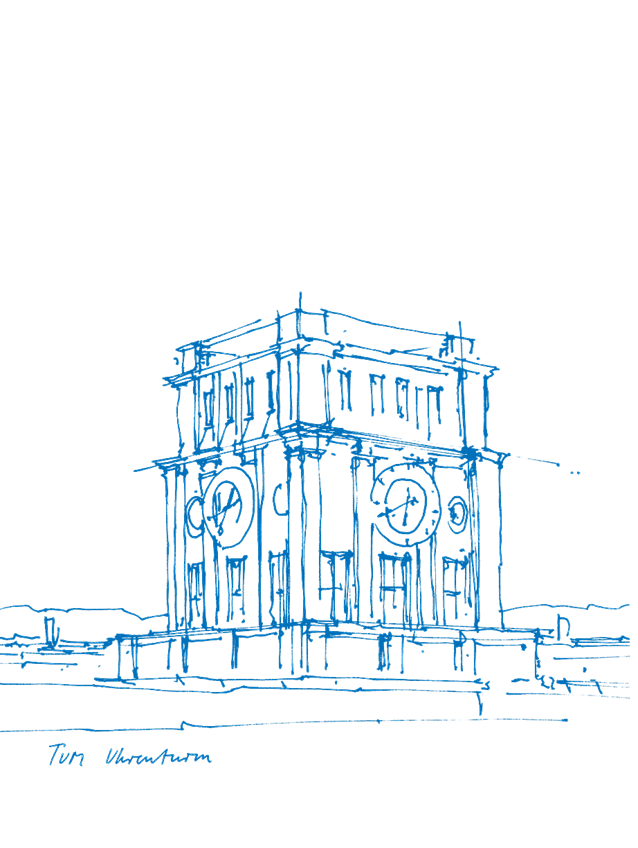
\includegraphics[width=.4\textwidth]{pics/TUM_Uhrenturm.png}};
%  \end{tikzpicture}
  \centering%
  \Large%
  \strut\textcolor{TUMBlue}{\inserttitle}%
  \\[4ex]%
  \normalsize%
  \strut\insertauthor%
  \\[2ex]%
  \footnotesize%
  \insertdate%
  \\[4ex]%
  \ifdefined\departmentname%
    \ifdefined\chairname%
      \chairname\\%
    \fi%
    \departmentname\\%
  \fi%
  \TUMname\\%
\end{frame}

  \begin{frame}[c,noframenumbering]
%    \begin{tikzpicture}[overlay,remember picture]
%      \node[opacity=0.5,anchor=south east] at ($(current page.south east)+(-1,-1)$) {%
%    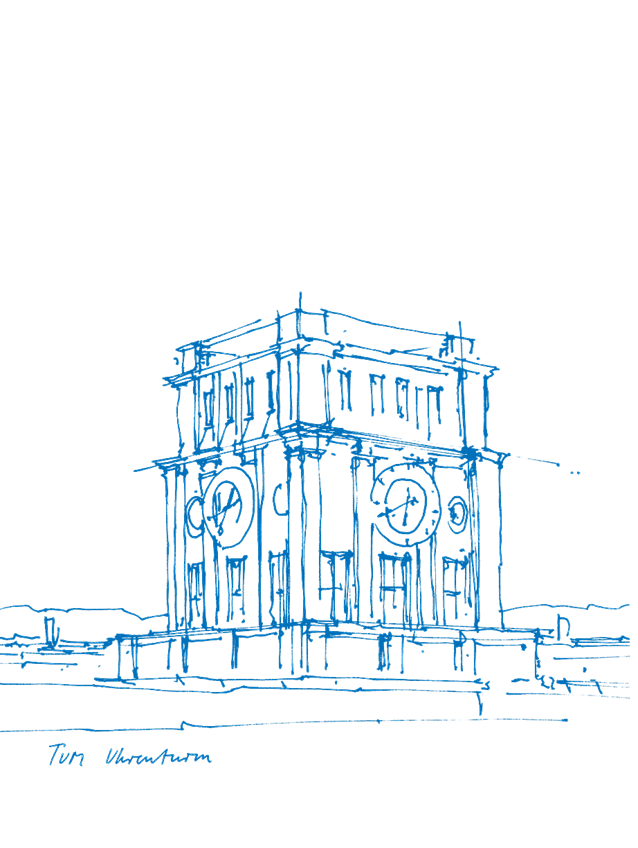
\includegraphics[width=.4\textwidth]{pics/TUM_Uhrenturm.png}};
%  \end{tikzpicture}
  \centering%
  \Large%
  \strut\textcolor{TUMBlue}{\inserttitle}%
  \\[4ex]%
  \normalsize%
  \strut{}\bfseries Paul Emmerich$^1$, Simon Ellmann$^2$, Sebastian Voit$^3$,\\ Fabian Bonk$^4$, Alex Egger$^5$, Alexander Frank$^6$, Thomas Günzel$^7$,\\ Stefan Huber$^8$, Maximilian Pudelko$^9$, Maximilian Stadlmeier$^{10}$ \normalfont %
  \\[2ex]%
  \footnotesize%
  $^1$C, thesis advisor\hspace{1em}
  $^2$Rust\hspace{1em}
  $^3$Go\hspace{1em}
  $^4$OCaml\hspace{1em}
  $^5$Haskell\hspace{1em}\\
  $^6$Latency measurements\hspace{1em}
  $^7$Swift\hspace{1em}
  $^8$IOMMU\hspace{1em}
  $^9$VirtIO driver\hspace{1em}
  $^{10}$C\#\hspace{1em}
  \\[4ex]%
    \ifdefined\departmentname%
    \ifdefined\chairname%
      \chairname\\%
    \fi%
    \departmentname\\%
  \fi%
  \TUMname\\%
\end{frame}
\setbeamertemplate{footline}[tumfootline]

\begin{frame}{About us}
\begin{columns}
\begin{column}{0.8\textwidth}
\emph{Paul}
\begin{itemize}
\item PhD student at Technical University of Munich
\item Researching performance of packet processing systems
\end{itemize}
\vfill
\emph{Simon}
\begin{itemize}
\item Rust driver as bachelor's thesis, now HiWi/research assistant
\end{itemize}
\emph{Sebastian}
\begin{itemize}
\item Rust driver as bachelor's thesis
\end{itemize}
\emph{Everyone else}
\begin{itemize}
\item Did a thesis with Paul as advisor
\end{itemize}
\end{column}
\begin{column}{0.15\textwidth}
%\begin{tikzpicture}[remember picture,overlay]
%	\node[xshift=-2.5cm,yshift=-3cm] at (current page.north east) {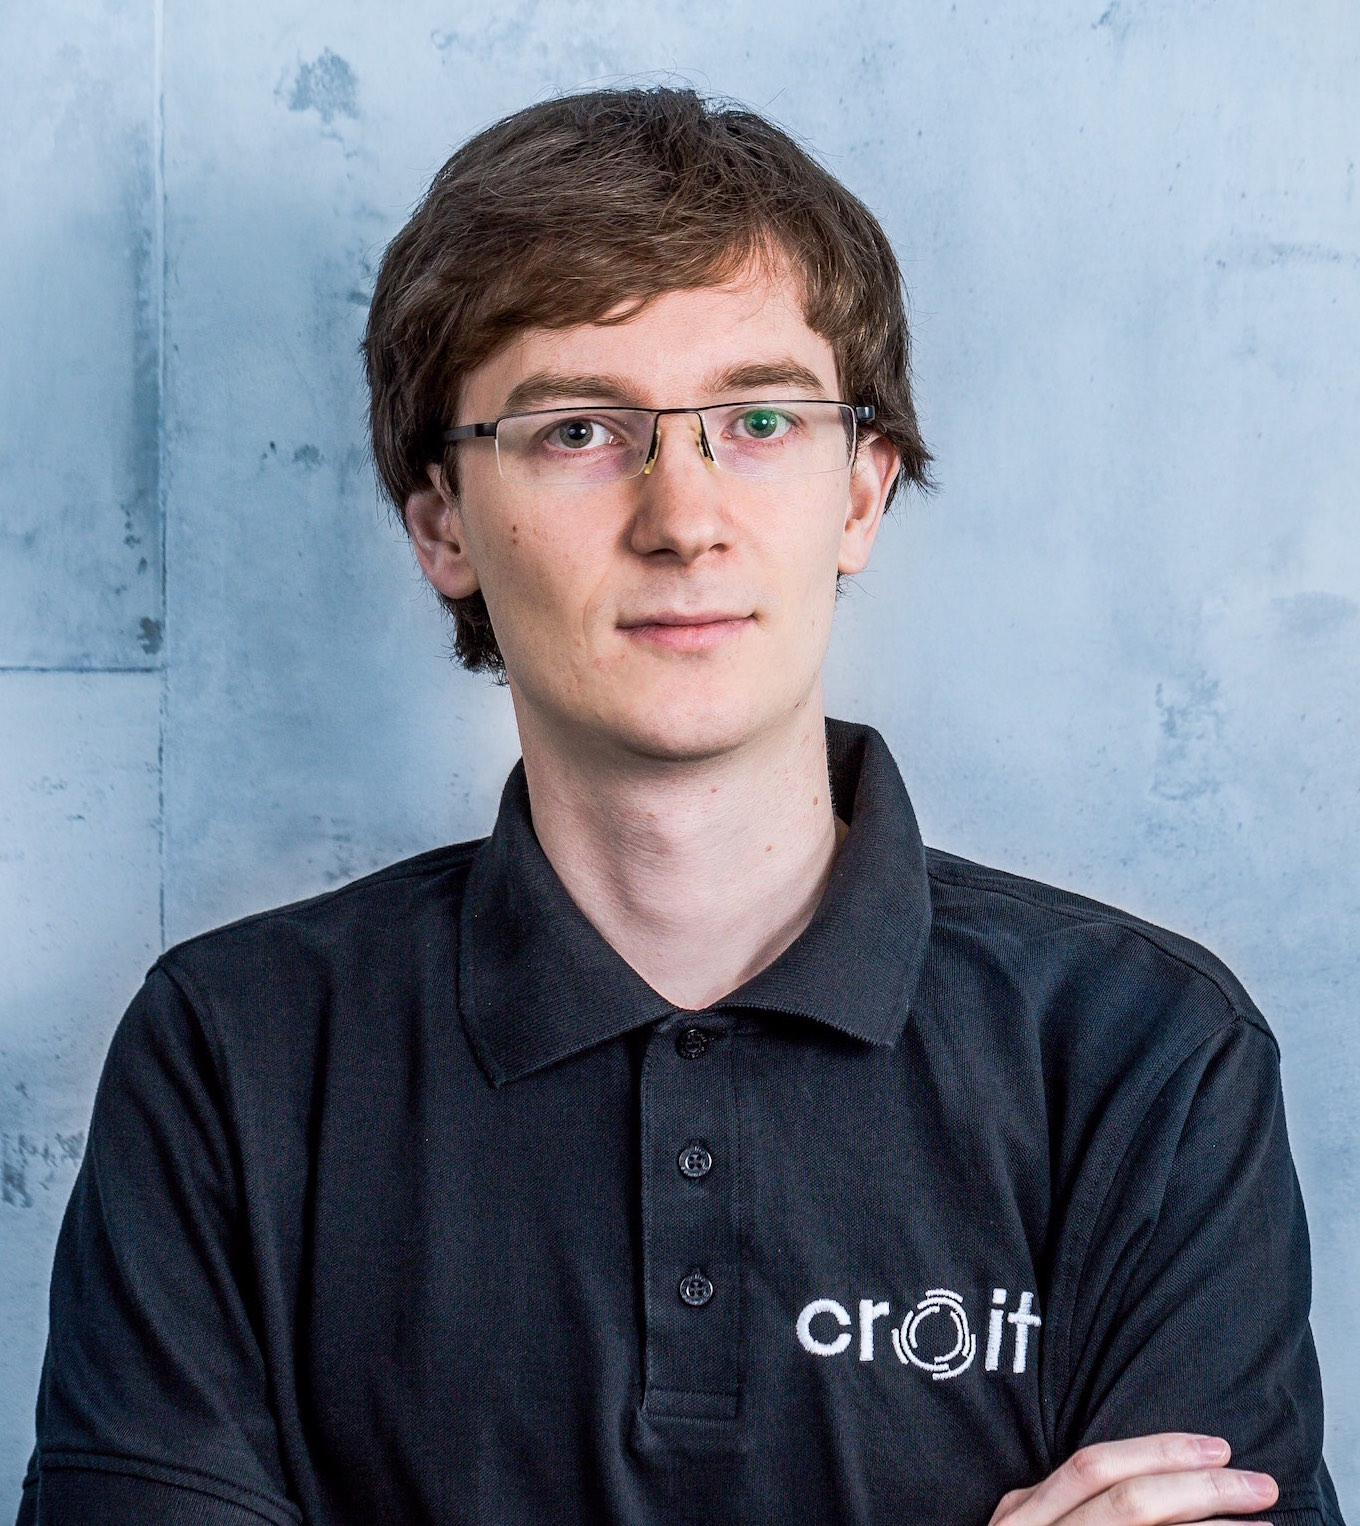
\includegraphics[width=0.2\textwidth]{pics/paul.jpg}};
%	\node[xshift=-2.5cm,yshift=-3cm] at (current page.south east) {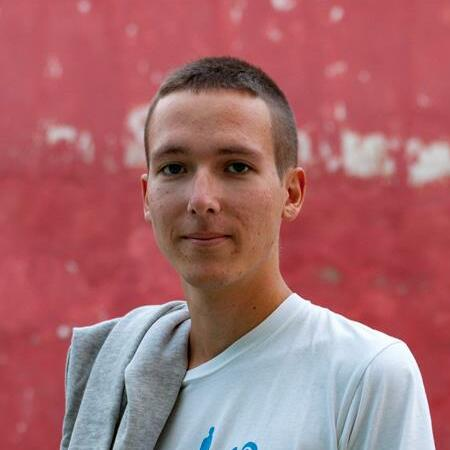
\includegraphics[width=0.2\textwidth]{pics/simon.jpg}};
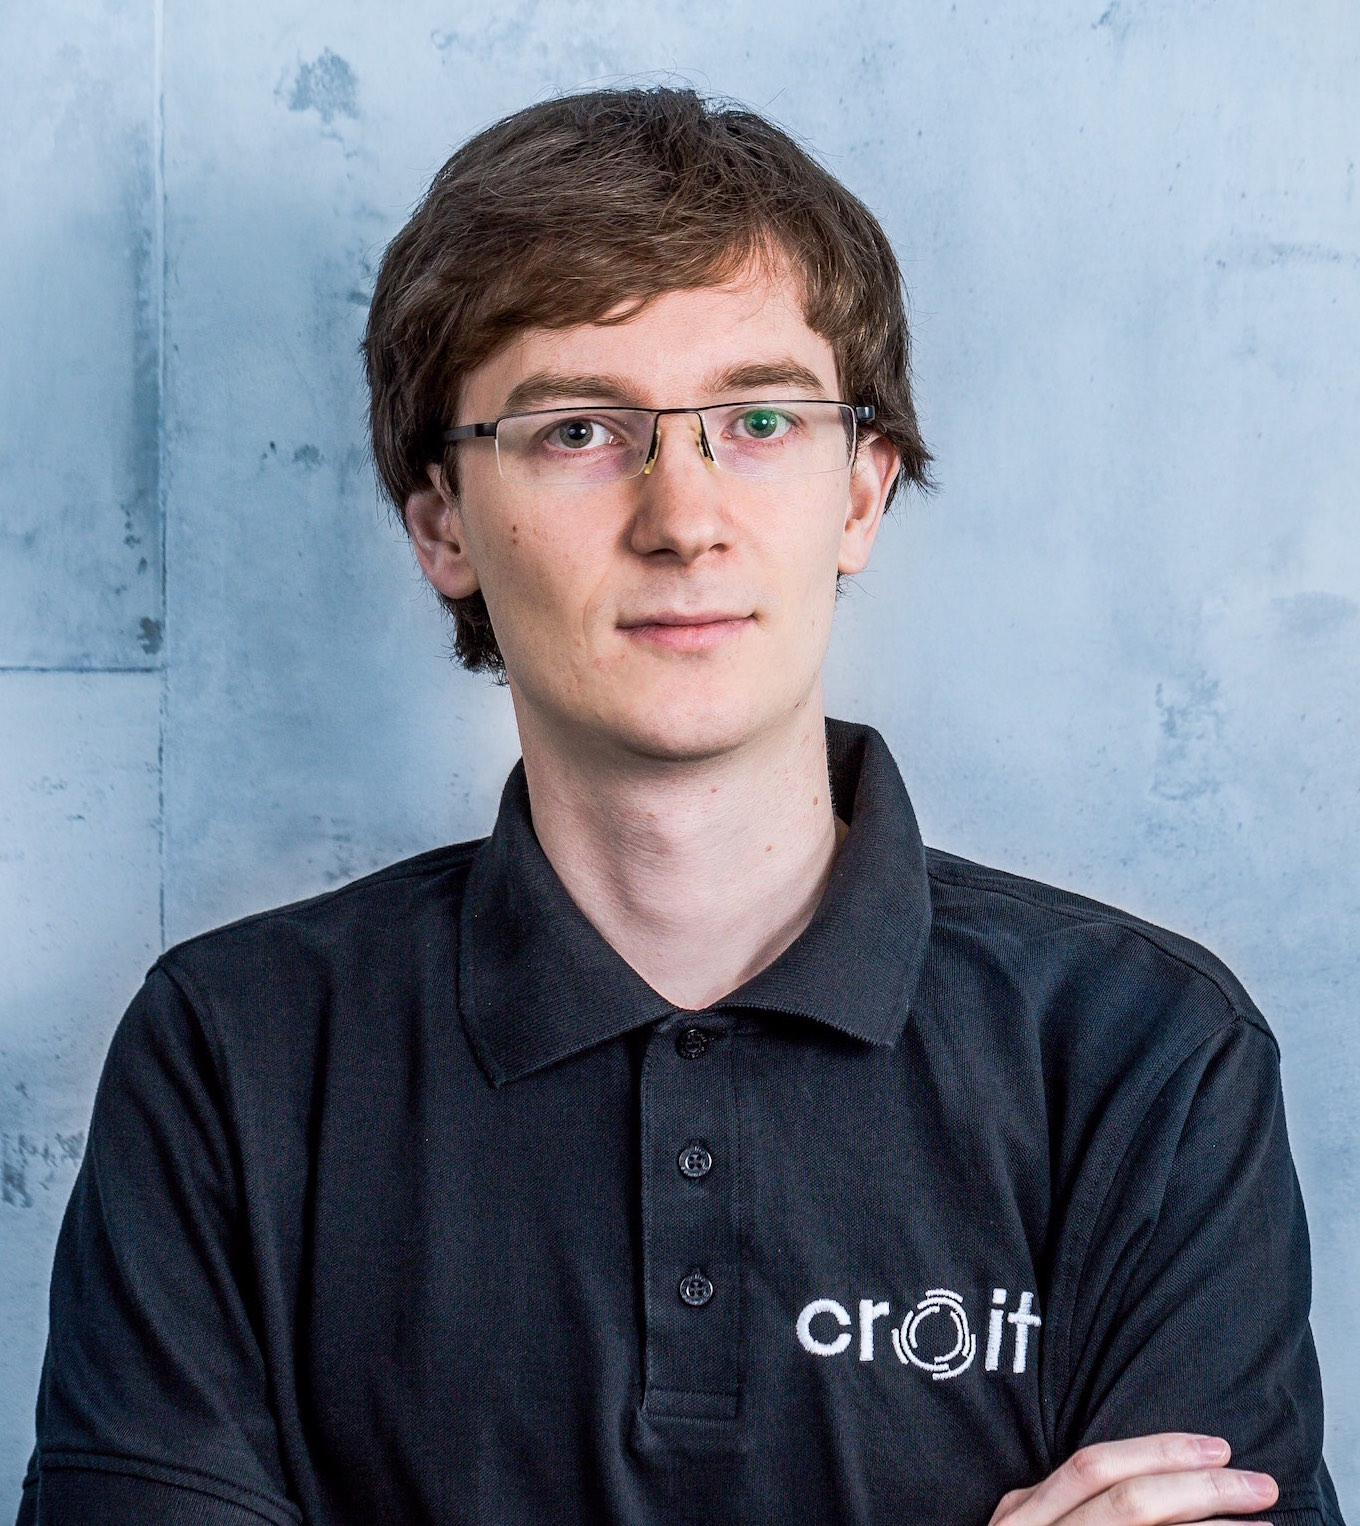
\includegraphics[width=0.8\textwidth]{pics/paul.jpg}\\
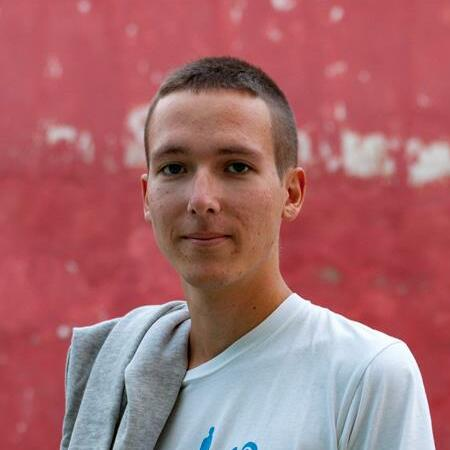
\includegraphics[width=0.8\textwidth]{pics/simon.jpg}\\
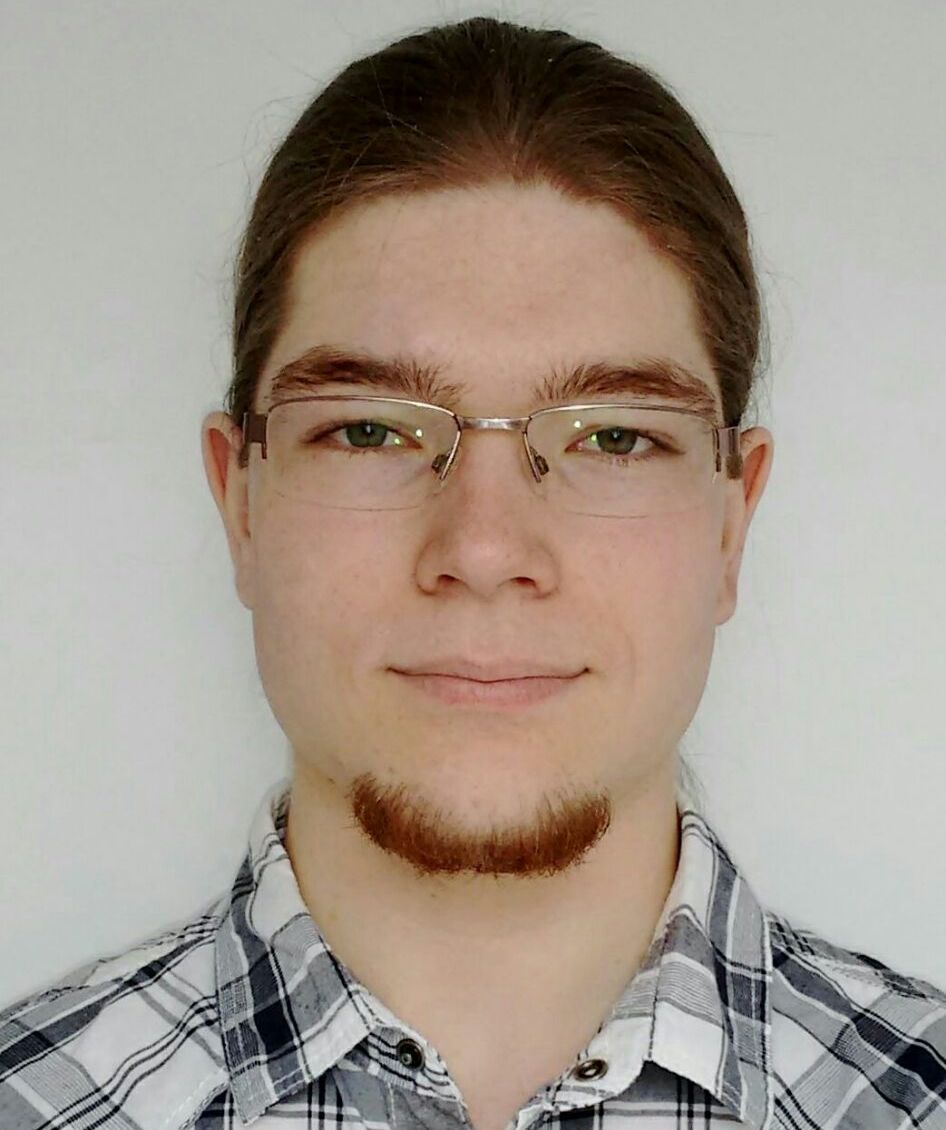
\includegraphics[width=0.8\textwidth]{pics/sebastian.jpg}
%\end{tikzpicture}
\end{column}
\end{columns}
\end{frame}


\begin{frame}{Network drivers}
\centering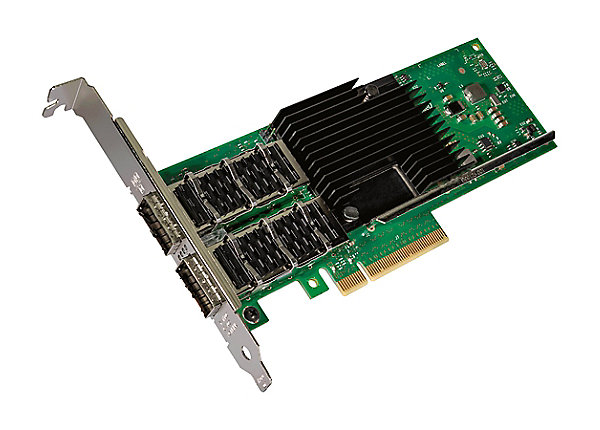
\includegraphics[width=0.60\textwidth]{pics/nic3}\\
\vspace{-1em}\tiny{Intel XL710 [Picture: Intel.com]}
\end{frame}

\begin{frame}{The ixy project}
\begin{itemize}
\item Attempt to write a simple yet fast user space network driver
\item It's a user space driver you can easily understand and read
\item $\approx$ 1,000 lines of C code, full of references to datasheets and specs
\item Supports Intel ixgbe NICs (82599, X540, Xeon D, ...)
\item New: supports VirtIO NICs (qemu/kvm and VirtualBox, we got a Vagrant setup!)
\item Check it out on GitHub: \url{https://github.com/emmericp/ixy}
\end{itemize}
\end{frame}


\begin{frame}{Expectation: Beautiful C code}
\begin{itemize}
\item Why write a driver in C?
\pause
\vspace{1em}
\item Most drivers are written in C
\item C is the lowest common denominator of systems programming languages
\item Everyone can read C?
\item C code can be beautiful
\end{itemize}
\end{frame}

\begin{frame}[fragile]{Reality: C can be ugly}
\begin{minted}[autogobble]{c}
#define mystery_macro(ptr, type, member) ({\
	const typeof(((type*)0)->member)* __mptr = (ptr);\
	(type*)((char*)__mptr - offsetof(type, member));\
})
\end{minted}
\end{frame}

\begin{frame}[fragile]{Reality: C can be ugly}
\begin{minted}[autogobble]{c}
#define container_of(ptr, type, member) ({\
	const typeof(((type*)0)->member)* __mptr = (ptr);\
	(type*)((char*)__mptr - offsetof(type, member));\
})
\end{minted}
\end{frame}


\begin{frame}[fragile]{Reality: C can be ugly}
\begin{minted}[autogobble]{c}
#define container_of(ptr, type, member) ({\
	const typeof(((type*)0)->member)* __mptr = (ptr);\
	(type*)((char*)__mptr - offsetof(type, member));\
})
\end{minted}
\begin{itemize}
\item Allows some ``inheritance'' in C to abstract driver implementations
\item Virtually all C drivers use this macro
\item The Linux kernel contains $\approx$ 15,000 uses of this macro
\end{itemize}
\end{frame}


%\setbeamertemplate{footline}{}
\begin{frame}{Reality: C can cause security problems}
%\centering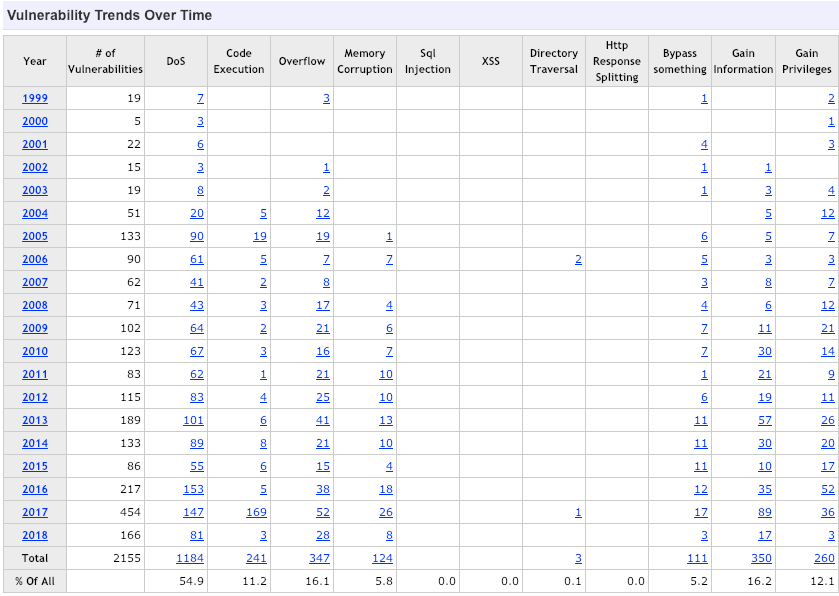
\includegraphics[width=0.65\textwidth]{pics/cve}\\
%\footnotesize bla subtitle
\begin{itemize}
\item blah biscuit paper \footnote{Biscuit}
\item ?? bugs
\item 40 due to memory safety
\vspace{1em}
\item How many of these are in drivers?
\pause
\item 39 are in drivers
\item (13 of these in Qualcomm WiFi driver)
\end{itemize}
\end{frame}
%\setbeamertemplate{footline}[tumfootline]

\begin{frame}{Should you really write new code in C in 2019?}
\begin{itemize}
\item If you have a choice: probably not, no
\pause
\item User space drivers can be written in \emph{any} language!
\item But are all languages an equally good choice?
\item Can high-level languages prevent bugs?
\item Is a JIT compiler or a garbage collector a problem in a driver?
\end{itemize}
\end{frame}

\setbeamertemplate{footline}{}
\begin{frame}{}
\centering
\includegraphics[width=0.65\textwidth]{pics/allthe1}
\end{frame}

\begin{frame}{}
\centering
\includegraphics[width=0.65\textwidth]{pics/allthe2}
\end{frame}

\begin{frame}{}
\centering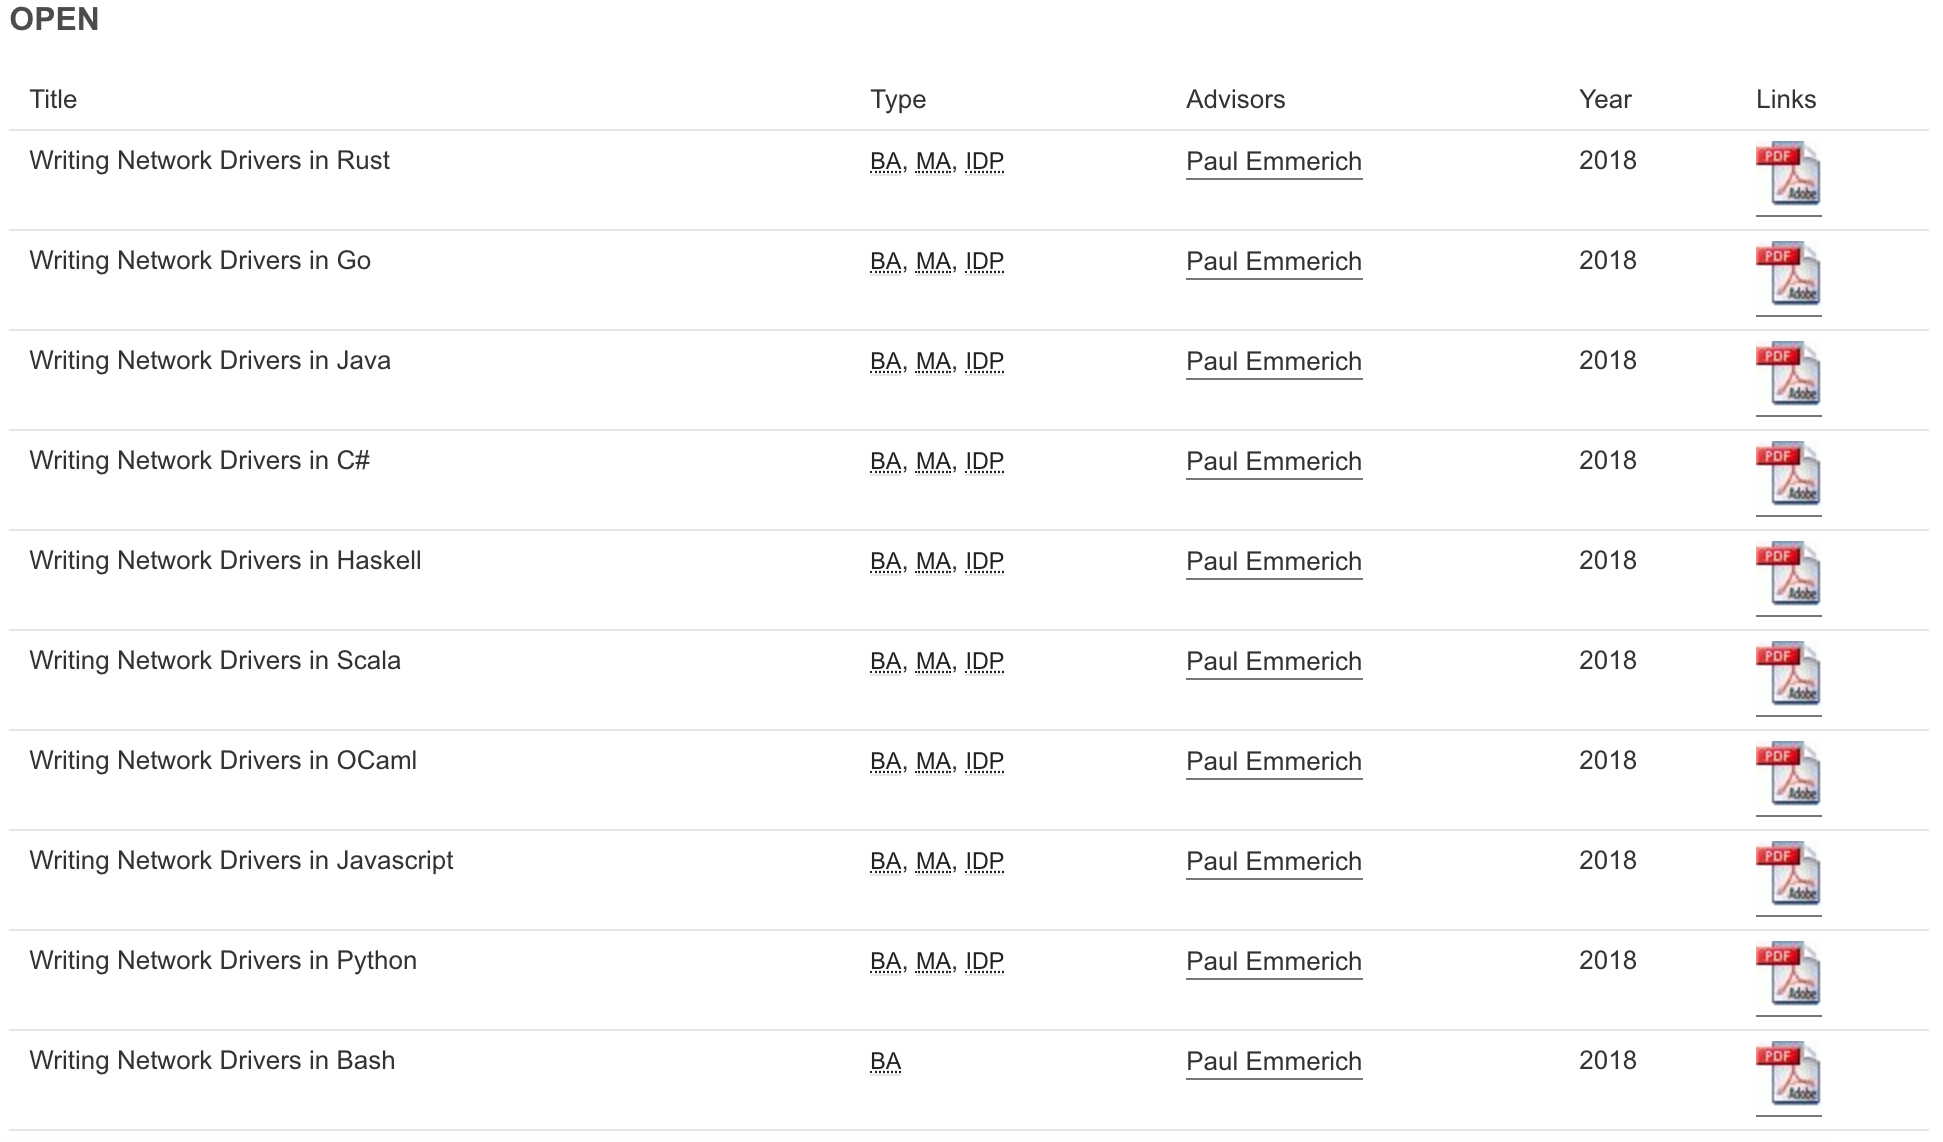
\includegraphics[width=0.85\textwidth]{pics/theses}
\end{frame}
\setbeamertemplate{footline}[tumfootline]


\begin{frame}{PCIe basics}
\begin{itemize}
\item MMIO
\item DMA
\item Interrupts
\end{itemize}
\end{frame}



\begin{frame}{How to write a user space driver in 4 simple steps}
\begin{itemize}
\item[1.] Unload kernel driver
\item[2.] \texttt{mmap} the PCIe MMIO address space
\item[3.] Figure out physical addresses for DMA
\item[4.] Write the driver
\end{itemize}
\end{frame}


\begin{frame}{Challenges for high-level languages}
\begin{itemize}
\item Access to \texttt{mmap} with the proper flags
\item Handle externally allocated memory in the language
\item Handle memory layouts/formats (i.e., access memory that looks like a given C struct)
\item Memory access semantics: memory barriers, volatile read/writes
\vspace{1em}
\pause
\item high-level unsafe blabla
\end{itemize}
\end{frame}



\begin{frame}{C\#}
\end{frame}

\begin{frame}{Swift}
%\centering\includestandalone[scale=0.79]{figures/benchmarks-swift-alone}
%\centering\includestandalone[scale=0.82]{figures/benchmarks-swift-with-c}
%\centering\includestandalone[scale=0.77]{figures/benchmarks-swift-batching}
\end{frame}

\begin{frame}{OCaml}
\end{frame}

\begin{frame}{Haskell}
\end{frame}

\begin{frame}{Go}
\begin{itemize}
\item Compiled programming language developed by Google 
\item General purpose language but designed for distributed systems
\item<2-> A driver is not a distributed system
\item<3-> Then why even use Go?
\begin{itemize}
\item<4-> Runtime for:\\Garbage Collection\\Memory \& Type safety
%\item<4-> Simple yet powerful concurrency via goroutines	%not relevant ofr a single core driver
\item<4-> Large standard library
\end{itemize}
\end{itemize}
\end{frame}

\begin{frame}{Go for Drivers}
\begin{itemize}
\item Actually a lot like C in many aspects
%maybe include some code examples?
\item<2-> Main differences:
\begin{itemize}
\item<2-> No pointer arithmetic (managing DMA memory)
\item<2-> No volatile (memory barriers for register access)
\end{itemize}
\item<3-> What we do instead:
\begin{itemize}
\item<3-> Manage DMA memory via slices
\item<3-> Unsafe pointers: circumvent runtime\\
	$\rightarrow$ Physical address calculation \& with atomic.Load/Store register access
\item<3-> Ruleset for unsafe pointers to still be valid
\end{itemize}
\end{itemize}
\end{frame}

\begin{frame}{Rust}
\begin{itemize}
\item compiled systems programming language
\item aims to be memory safe (especially regarding concurrency), i.e.
\begin{itemize}
\item no race conditions,
\item no dangling pointers,
\item no undefined behaviour,
\item ...
\end{itemize}
\item unique ownership system and ruleset for moving/borrowing values
%\item highly efficient through zero-cost abstractions
\end{itemize}
\end{frame}

\begin{frame}{Rust's Ownership System}
\begin{itemize}
\item Three simple rules:
\begin{itemize}
\item Each value has a variable that is its owner.
\item There can only be one owner at a time.
\item When the owner goes out of scope, the value is freed.
\end{itemize}
\item Rules are enforced at compile-time
\item Ownership can be passed to another variable% by
%\begin{itemize}
%\item ``moving'' the value or by
%\item ``borrowing'' it through a reference
%\end{itemize}
\end{itemize}
\end{frame}

\begin{frame}{Rust: Safe vs. Unsafe}
\begin{itemize}
\item not everything can be done in safe Rust
\item calling foreign functions and dereferencing raw pointers is always unsafe
\item many functions in Rust's standard library make use of unsafe code
\end{itemize}
\end{frame}

\begin{frame}[fragile]{Rust}
\begin{itemize}
\item biggest challenge: memory handling inside and outside the driver
\end{itemize}
\begin{minted}{c}
fn set_reg32(&self, reg: u32, val: u32) {
  assert!(
    reg as usize <= self.len - 4 as usize,
    "memory access out of bounds"
  );

  unsafe {
    ptr::write_volatile((self.addr as usize + reg as usize) as *mut u32, val);
  }
}
\end{minted}
\end{frame}

\begin{frame}[fragile]{Rust}
% TODO: some packet code or graphic? forwarder?
\begin{itemize}
\item look at this nice code ...
\end{itemize}
\begin{minted}{c}
fn set_reg32(&self, reg: u32, val: u32) {
  assert!(
    reg as usize <= self.len - 4 as usize,
    "memory access out of bounds"
  );

  unsafe {
    ptr::write_volatile((self.addr as usize + reg as usize) as *mut u32, val);
  }
}
\end{minted}
\end{frame}

\begin{frame}{Performance comparison}
\centering\includestandalone[scale=0.82]{figures/benchmarks-all-throughput}
\end{frame}

\begin{frame}{Batching}
\centering\includestandalone[scale=0.85]{figures/benchmarks-all-batching}
\end{frame}

\begin{frame}{Performance comparison}
% TODO: observations and reasons/speculations for good/bad performance?
\begin{itemize}
\item Rust's throughput close to C, safe wrappers lead to more memory operations
\item Swift performs incredibly poor
\item ...
\end{itemize}
\end{frame}

\begin{frame}{Garbage collection and JIT compilation vs. latency}
\end{frame}


\begin{frame}{Restricting devices with the IOMMU}
\end{frame}

\begin{frame}{Look ma, no root}
\end{frame}


\begin{frame}{Why to write a user space network driver?}
\end{frame}

\begin{frame}{(Maybe) network stack of the future}
\end{frame}

\begin{frame}{Why? Features!}
\end{frame}

\begin{frame}{Example: hardware timestamping}
\end{frame}


\begin{frame}{Conclusion: Check out our code}
%\centering \qrcode[height=3cm]{https://github.com/ixy-languages/ixy-languages}
\begin{itemize}
\item Meta-repository with links: \url{https://github.com/ixy-languages/ixy-languages}
\item Drivers are simple: don't be afraid of them
\item No kernel code needed :)
\end{itemize}
%\centering \Huge Q \& A
\end{frame}













\begin{frame}{What I care about}
\centering\begin{tikzpicture}[scale=1.35]
	\foreach \x in {1,2,...,7} {
		\pgfmathparse{40 - \x*5}\let\layershade\pgfmathresult
		\pgfmathparse{\x/2}\let\y\pgfmathresult
		\def\layercolor{TUMDarkerBlue}
		\draw[line width=.5pt,fill=\layercolor!\layershade]
			(0,\y) rectangle ($(4,\y+0.5)$);

	}
	\foreach \x in {1,2,...,7} {
		\node at (0.17,0.25+\x*0.5) {\fontsize{5}{6}\selectfont\bf \x};
	}
	\node at (2,0.75) {\fontsize{7}{8}\selectfont Physical};
	\node at (2,1.25) {\fontsize{7}{8}\selectfont Data Link};
	\node at (2,1.75) {\fontsize{7}{8}\selectfont Network};
	\node at (2,2.25) {\fontsize{7}{8}\selectfont \cancel{Transport}};
	\node at (2,2.75) {\fontsize{7}{8}\selectfont \cancel{Session}};
	\node at (2,3.25) {\fontsize{7}{8}\selectfont \cancel{Presentation}};
	\node at (2,3.75) {\fontsize{7}{8}\selectfont \cancel{Application}};
\end{tikzpicture}
\end{frame}


\begin{frame}{Not all apps run on top of HTTP}
Lots of network functionality is moving from specialized hardware to software:
\begin{itemize}
\item Routers
\item (Virtual) Switches
\item Firewalls
\item Middleboxes
\end{itemize}
Buzzwords: Network Function Virtualization, Service Function Chaining
\end{frame}

\begin{frame}{Example application}
%\centering\includestandalone{figures/softwarearch-simple}
\end{frame}


\begin{frame}{Normal applications}
%\centering\includestandalone{figures/softwarearch-classic}
\end{frame}

\begin{frame}{What it really looks like}
%\centering\includestandalone{figures/softwarearch-dragons}
\end{frame}

\begin{frame}{Performance}
\begin{itemize}
\item Packets per second on a 10\,Gbit/s link: up to \emph{14.88\,Mpps}
\item<2-> Packets per second on a 100\,Gbit/s link: up to \emph{148.8\,Mpps}
\item<3-> Clock cycles per packet on a 3\,GHz CPU with 14.88\,Mpps: $\approx 200$ cycles
\item<3-> Typical performance target: $\approx$ 5 to 10\,Mpps per CPU core for simple forwarding
\end{itemize}
\end{frame}

\begin{frame}{Performance: User space app}
\begin{itemize}
\item<1-> Typical performance target: $\approx$ 5 to 10\,Mpps per CPU core for simple forwarding
\item<1-> 5 to 10\,Mpps $=$ \emph{300 to 600 cycles} per packet at 3\,GHz
\vspace{1em}
\item<2-> Time to cross the user space boundary: very very long
\vspace{1em}
\item<3-> Single-core forwarding performance with sockets: $\approx$ 0.3\,Mpps
\item<3-> Single-core forwarding performance with libpcap: $\approx$ 1\,Mpps
%\item Latency of a typical hardware switch: $\le 1\,\mu s$
%\item Latency of a hardware switch: $\le 1\,\mu s$
\end{itemize}
\end{frame}

%\begin{frame}{Performance dragons?}
%\centering\includestandalone{figures/softwarearch-dragons}
%\end{frame}

\begin{frame}{Move the application into the kernel}
\centering\includestandalone{figures/softwarearch-kernel}
\end{frame}

\begin{frame}{Move the application into the kernel}
New problems:
\begin{itemize}
\item Cumbersome to develop
\item Usual kernel restrictions (e.g., C as programming language)
\item Application can (and will) crash the kernel
\end{itemize}
\end{frame}

\begin{frame}{Performance: Kernel app}
\begin{itemize}
\item<1-> Typical performance target: $\approx$ 5 to 10\,Mpps per CPU core for simple forwarding
\item<1-> 5 to 10\,Mpps $=$ \emph{300 to 600 cycles} per packet at 3\,GHz
\vspace{1em}
\item<2-> Time to receive a packet in the Linux kernel: $\approx \emph{500}$ \emph{cycles}
\item<3-> Time to send a packet in the Linux kernel: $\approx \emph{440}$ \emph{cycles}
\item<4-> Time to allocate, initialize, and free a \texttt{sk\_buff} in the Linux kernel: $\approx \emph{400}$ \emph{cycles}
\vspace{1em}
\item<5-> Single-core forwarding performance with Open vSwitch: $\approx$ 2\,Mpps
\item<5-> Hottest topic in the Linux kernel: XDP, which fixes some of these problems
\end{itemize}
\end{frame}


\begin{frame}{Do more in user space?}
%\centering\includestandalone{figures/softwarearch-moreuserspace}
\end{frame}

\begin{frame}{User space packet processing frameworks}
Examples for such frameworks
\begin{itemize}
\item netmap
\item PF\_RING ZC
\item pfq
\end{itemize}
\end{frame}

\begin{frame}{Problems}
\begin{itemize}
\item Non-standard API, custom kernel module required
\item Most frameworks require patched drivers
\item Exclusive access to the NIC for one application
\item No access to the usual kernel features
\begin{itemize}
\item Limited support for kernel integration in netmap
\end{itemize}
\item Poor support for hardware offloading features of NICs
\item Framework needs explicit support for each NIC, limited to a few NICs
\end{itemize}
\end{frame}

\begin{frame}{Do even more in user space?}
%\centering\includestandalone{figures/softwarearch-fulluserspace}
\end{frame}

\begin{frame}{User space driver frameworks}
Examples for such frameworks
\begin{itemize}
\item DPDK
\item Snabb
\end{itemize}
\end{frame}

\begin{frame}{Problems}
\begin{itemize}
\item Non-standard API
\item Exclusive access to the NIC for one application
\item Framework needs explicit support for each NIC model
\begin{itemize}
\item DPDK supports virtually all $\ge$ 10\,Gbit/s NICs
\end{itemize}
\item Limited support for interrupts
\begin{itemize}
\item Interrupts not considered useful at $\ge$ 0.1\,Mpps
\end{itemize}
\item No access to the usual kernel features
\end{itemize}
\end{frame}


\begin{frame}{Hardware: Intel \texttt{ixgbe} family (10\,Gbit/s)}
\begin{itemize}
\item \texttt{ixgbe} family: 82599ES (aka X520), X540, X550, Xeon D embedded NIC
\item Commonly found in servers or as on-board chips
\item Very good datasheet publicly available
%\vspace{1em}
\item Almost no logic hidden behind black-box firmware
%\item<2-> Black-box firmware contains almost no magic
%\item<2-> Drivers for many newer NICs often just exchanges messages with the firmware
%\item<2-> Here: all hardware features directly exposed to the driver
\end{itemize}
\end{frame}


\newmintinline[ccode]{c}{}
\newmintinline[bashcode]{c}{}

\begin{frame}[fragile=singleslide]{Find the device we want to use}
\begin{Verbatim}[commandchars=\\\{\}]
# lspci
03:00.0 Ethernet controller: Intel Corporation 82599ES 10-Gigabit SFI/SFP+ ...
03:00.1 Ethernet controller: Intel Corporation 82599ES 10-Gigabit SFI/SFP+ ...
\end{Verbatim}
\end{frame}

\begin{frame}[fragile=singleslide]{Find the device we want to use}
\begin{Verbatim}[commandchars=\\\{\}]
# lspci
\textbf{03:00.0} Ethernet controller: Intel Corporation 82599ES 10-Gigabit SFI/SFP+ ...
\textbf{03:00.1} Ethernet controller: Intel Corporation 82599ES 10-Gigabit SFI/SFP+ ...
\end{Verbatim}
\end{frame}

\begin{frame}[fragile=singleslide]{Unload the kernel driver}
\begin{minted}{bash}
echo 0000:03:00.1 > /sys/bus/pci/devices/0000:03:00.1/driver/unbind
\end{minted}
%\begin{itemize}
%\item \ccode{asdf hi}
%\item \ccode|asdf|
%\item \mintinline{c}{hi}
%\end{itemize}
\end{frame}

\begin{frame}[fragile=singleslide]{\texttt{mmap} the PCIe configuration address space from user space}
\begin{minted}[autogobble]{c}
	int fd = open("/sys/bus/pci/devices/0000:03:00.0/resource0", O_RDWR);
	struct stat stat;
	fstat(fd, &stat);
	uint8_t* registers = (uint8_t*) mmap(NULL, stat.st_size, PROT_READ | PROT_WRITE,
	                                     MAP_SHARED, fd, 0);
\end{minted}
\end{frame}



\end{document}

